% !TEX root = ./article.tex

\documentclass[spanish]{article}

\usepackage{mystyle}
\usepackage{myvars}
\usepackage{mylinearprogramming}



%-----------------------------

\begin{document}

	\maketitle % Insert title

	\thispagestyle{fancy} % All pages have headers and footers


%-----------------------------
%	ABSTRACT
%-----------------------------

	\begin{abstract}
		\noindent En este documento se realiza una descripción acerca del \emph{problema del viajante} (TSP), que consiste en la búsqueda del camino más corto que permita visitar un conjunto de nodos. Además se proporcionan distintas formulaciones para dicho problema así como un conjunto de heurísticas aproximadas que permiten su resolución de manera mucho menos costosa. También se presenta la descripción de la variante del \emph{problema del viajante con ventana de tiempo} (TSPTW), que se caracteriza por exigir que la visita de un determinado nodo se realice dentro de un intervalo temporal prefijado. Por último, se presentan las soluciones de distintos conjuntos de datos resultas mediantes las estrategias descritas en el documento.
	\end{abstract}

%-----------------------------
%	TEXT
%-----------------------------

	\section{Problema del Viajante (TSP)}

		\paragraph{}
		El \emph{Problema del Viajante} (o \emph{Travelling Salesman Problem (TSP)} en inglés) consiste en la búsqueda del camino más corto necesario para visitar un conjunto de $n$ nodos separados entre si por unas determinadas distancias $d_ij$. Esto es equivalente a la generación del ciclo hamiltoniano en un grafo cuyas aristas tienen determinados pesos (las distancias).

		\paragraph{}
		Para resolver este problema existen distintas formulaciones de manera exacta, entre las que se encuentran la formulación estandar de la ecuación \eqref{eq:tsp_basic}, la formulación de \emph{Tucker-Miller} descrita en la ecuación \eqref{eq:tsp_tm} o la resolución mediante el apoyo en un modelo de redes complementario tal y como se muestra en la ecuación \eqref{eq:tsp_redes}.

		\subsection{Formulaciones Exactas}

			\paragraph{}
			La formulación estándar o básica para el problema del viajante se muestra en la ecuación \eqref{eq:tsp_basic}, sin embargo esta tan solo es de interés a nivel teoríco debido al elevado número de restricciones que se generan en su modelización. Por tanto en la práctica se utilizan otras formulaciones que se describen a continuación.

			\begin{eqfloat}
				\begin{equation}
					\begin{array}{ll@{}ll}
						\text{Minimizar}	& \displaystyle\sum\limits_{i = 1}^{n}\sum\limits_{j}^{n} & d_{ij}x_{ij} &\\
						\text{sujeto a}		& \displaystyle\sum\limits_{i = 1}^{n}	&	x_{ij} 	= 1,  & \forall j \in \{1,...,n\}\\
															& \displaystyle\sum\limits_{j = 1}^{n}	&	x_{ij} 	= 1,  & \forall i \in \{1,...,n\}\\
															& \displaystyle\sum\limits_{i \in S, j \not\in S}	&	x_{ij} 	\geq 1,  & \forall S \subset N / S \neq \emptyset, S \neq N \\
															&                               &	x_{ij} \in \{0,1\}, 	& \forall i,j \in \{1,...,n\}
					\end{array}
				\end{equation}
				\caption{Formulación estándar para el \emph{problema del viajante (TSP)}.}
				\label{eq:tsp_basic}
			\end{eqfloat}


			\paragraph{}
			La formulación de redes consiste en la modificación de las restricciones derivadas del conjunto $S$ por un modelo de redes complementario a partir de las variables de decisión $y_{ij}$ de carácter real positivo así como las constantes $b_i$, que en conjunto generan un encadenamiento del camino, lo cual elimina la posibilidad de que se generen subtours. Esta modelización se puede visualizar en la ecuación \eqref{eq:tsp_redes}.

			\begin{eqfloat}
				\begin{equation}
					\begin{array}{ll@{}ll}
						\text{Minimizar}	& \displaystyle\sum\limits_{i = 1}^{n}\sum\limits_{j}^{n} & d_{ij}x_{ij} &\\
						\text{sujeto a}		& \displaystyle\sum\limits_{i = 1}^{n}	&	x_{ij} 	= 1,  & \forall j \in \{1,...,n\}\\
															& \displaystyle\sum\limits_{j = 1}^{n}	&	x_{ij} 	= 1,  & \forall i \in \{1,...,n\}\\
															& \displaystyle\sum\limits_{j = 1}^n	y_{ij} - &\displaystyle\sum\limits_{j = 1}^n	y_{ji} = b_{i},  & \forall i \in \{1,...,n\} \\
															&                               &	y_{ij}  \leq (n-1)x_{ij}, 	&  \forall i,j \in \{1,...,n\}\\
															&                               &	b_{1}  = n - 1, 	& \\
															&                               &	b_{i} = -1, 		& \forall i \in \{2,...,n\} \\
															&                               &	y_{ij} \geq 0, 		& \forall i,j \in \{1,...,n\} \\
															&                               &	x_{ij} \in \{0,1\}, 	& \forall i,j \in \{1,...,n\}
					\end{array}
				\end{equation}
				\caption{Formulación de Redes para els \emph{problema del viajante (TSP)}.}
				\label{eq:tsp_redes}
			\end{eqfloat}

			\paragraph{}
			La formulación propuesta por \emph{Tucker-Miller} se apoya en la existencia de las variables de decisión $u_i$ de carácter entero y positivo, que desempeñan la misma tarea que el modelo de redes complementario de la formulación anterior, es decir, la restricción que elimine la posibilidad de que se formen subtours. La formulación de \emph{Tucker-Miller} se muestra en la ecuación \eqref{eq:tsp_tm}.

			\begin{eqfloat}
				\begin{equation}
					\begin{array}{ll@{}ll}
						\text{Minimizar}	& \displaystyle\sum\limits_{i = 1}^{n}\sum\limits_{j}^{n} & d_{ij}x_{ij} &\\
						\text{sujeto a}		& \displaystyle\sum\limits_{i = 1}^{n}	&	x_{ij} 	= 1,  & \forall j \in \{1,...,n\} \\
															& \displaystyle\sum\limits_{j = 1}^{n}	&	x_{ij} 	= 1,  & \forall i \in \{1,...,n\} \\
															& 				&	u_i - u_j + n x_{ij}	\leq n-1,  & \forall i, j \in \{2,...,n\}, i \neq j \\
															&                               &	u_{i} \in \{2,...,n\}, 		& \forall i \in \{2,...,n\} \\
															&                               &	u_{1}  = 1, 	& \\
															&                               &	x_{ij} \in \{0,1\}, 	& \forall i,j \in \{1,...,n\}
					\end{array}
				\end{equation}
				\caption{Formulación de Tucker-Miller para el \emph{problema del viajante (TSP)}.}
				\label{eq:tsp_tm}
			\end{eqfloat}


			\paragraph{}
			La resolución del problema del viajante mediante la optimización exacta de los modelos descritos anteriormente conlleva un gran coste computacional derivado de la dificultad por la explosión combinatoria que se produce cuando el número de nodos del conjunto de datos crece. Por lo tanto, existen alternativas que ofrecen resultados aproximados mediante distintas heurísticas que reducen de manera drástica el tiempo de cómputo. Entre ellas se encuentran la heurística del \emph{Entorno más Cercano}, \emph{2-opt}, \emph{GRASP} y \emph{Simulated Anneling}, que se describen a continuación.

		\subsection{Estrategia Entorno más Cercano}

			\paragraph{}
			La heurística del entorno más cercano se muestra en la figura \ref{code:tsp-greedy}. Consiste en una estrategia iterativa que trata de minimizar el error relativo durante cada iteracción (seleccionando el nodo más cercano al actual) hasta formar un camino que visite todos los nodos del conjunto de datos.

			\begin{figure}
	      \centering
	      \BVerbatimInput{code/tsp-greedy.pseudo}
	      \caption{Heurística del \emph{Entorno más Cercano}}
	      \label{code:tsp-greedy}
	    \end{figure}

		\subsection{Estrategia 2-OPT}

			\paragraph{}
			La herística 2-opt se muestra en la figura \ref{code:tsp-2-opt}. Esta estrategia consiste en una mejora sobre la del entorno más cercano, que se apoya en una solución inicial de la misma para después tratar de mejorarla buscando la minimización de la distancia total mediante el intercambio de índices entre los nodos del camino. Se realiza dicha acción hasta que el camino no se puede minimizar más mediante dicha estrategia (por entrar en un mínimo local).

			\begin{figure}
	      \centering
	      \BVerbatimInput{code/tsp-2-opt.pseudo}
	      \caption{Heurística \emph{2-opt}}
	      \label{code:tsp-2-opt}
	    \end{figure}

		\subsection{Estrategia GRASP}

			\paragraph{}
			La heurística GRASP se muestra en la figura \ref{code:tsp-grasp}. Esta se apoya en las estrategias anteriores pero añade aleatoriedad en el punto de selección del nodo más próximo, selecionando uno al azar de entre los $k$ más próximos. Para mejorar la precisión en los resultados realiza esta acción durante $N$ iteracciónes y selecciona el camino que minimiza la distancia de entre totas las soluciones obtenidas.

			\begin{figure}
				\centering
				\BVerbatimInput{code/tsp-grasp.pseudo}
				\caption{Heurística \emph{GRASP}}
				\label{code:tsp-grasp}
			\end{figure}

		\subsection{Estrategia Simulated Anneling}

			\paragraph{}
			La heurística Simulated Anneling se muestra en la figura \ref{code:tsp-simulated-anneling}. Dicha estrategia es similar a la $2-opt$ descrita anteriormente. Sin embargo, esta se apoya en ideas extraídas del sector de la metalurgia, en el cual se realiza un enfriamiento de manera suavizada de los metales para tratar de mejorar su resistencia. En este caso se seleccionan dos nodos al azar y se intercambian los nodos subsiguientes a estos. Este cambio se fija si se reduce la distancia global del camino o de manera aleatoria en el caso de que no sea así. La probabilidad de que se cambie aleatoriamente se va decrementando mediante un determinado factor llamado temperatura.

			\begin{figure}
	      \centering
	      \BVerbatimInput{code/tsp-simulated-anneling.pseudo}
				\caption{Heurística \emph{Simulated Anneling}}
	      \label{code:tsp-simulated-anneling}
	    \end{figure}

	\section{Problema del Viajante con Ventana de Tiempo (TSPTW)}

		\paragraph{}
		El problema del viajante con ventana de tiempo consiste en una variación respecto del problema básico que añade la restricción de visitar a los nodos en un determinado intervalo de tiempo prefijado mediante los valores $[a_i, b_i]$ para cada nodo. En la ecuación \eqref{eq:tsptw_tm} se muestra una modelización para dicho problema. Nótese que en este caso se ha utilizado como problema base la formulación descrita por Tucker-Miller para el problema del viajante, al cual se le han añadido las pertinentes restricciones para que se cumplan las ventanas de tiempo. Esto se ha llevado a cabo añadiento las variables de decisión $\beta_i$ de carácter real positivo, que se corresponden con el momento en que el nodo $i$ será visitado.

		\begin{eqfloat}
			\begin{equation}
				\begin{array}{ll@{}ll}
					\text{Minimizar}	& \displaystyle\sum\limits_{i = 1}^{n}\sum\limits_{j}^{n} & d_{ij}x_{ij} &\\
					\text{sujeto a}		& \displaystyle\sum\limits_{i = 1}^{n}	&	x_{ij} 	= 1,  & \forall j \in \{1,...,n\} \\
														& \displaystyle\sum\limits_{j = 1}^{n}	&	x_{ij} 	= 1,  & \forall i \in \{1,...,n\} \\
														& 				&	\beta_{i} + d_{ij} - M(1-x_{ij}) \leq \beta_{j},  & \forall i, j \in \{1,...,n\}, j \neq 1 \\
														& 				&	u_i - u_j + n x_{ij}	\leq n-1,  & \forall i, j \in \{2,...,n\}, i \neq j \\
														&                               &	u_{i} \in \{2,...,n\}, 		& \forall i \in \{2,...,n\} \\
														&                               &	u_{1}  = 1, 	& \\
														&                               &	a_{i} \leq \beta_{i}, 		& \forall i \in \{1,...,n\} \\
														&                               &	\beta_{i} \leq b_{i}, 		& \forall i \in \{1,...,n\} \\
														&                               &	x_{ij} \in \{0,1\}, 	& \forall i,j \in \{1,...,n\}
				\end{array}
			\end{equation}
			\caption{Formulación de Tucker-Miller para el \emph{problema del viajante con ventana de tiempo (TSPTW)}.}
			\label{eq:tsptw_tm}
		\end{eqfloat}

	\section{Resolución de Problemas}

		\paragraph{}
		En esta sección se presentan los resultados obtenidos tras resolver el problema del viajante (TSP) con distintos conjuntos de datos de entrada. Dichos resultados se han agrupado por problema en lugar de por estrategia de resolución, lo cual permite comparar de manera más simple cada una de ellas. En algunos casos estos conjuntos de datos se corresponden con coordenadas cartesianas, para lo cual es necesario calcular la distancias entre cada par de puntos, lo que permite realizar una representación gráfica de la solución. Sin embargo, en otros casos tan solo se suministran las distancias, por lo que la representación gráfica no es posible. Por último, se resuelven dos problemas con ventana de tiempo (TSPTW) de manera exacta, para el cual se suministran además los puntos de inicio y fin permitidos para visitar cada nodo.

		\subsection{burma14}

			\paragraph{}
			El conjunto de datos está formado por las coordenadas de $14$ nodos (por lo que es necesario calcular las distancias previamente). En este caso se resuelve de manera exacta mediante la formulación de \emph{Tucker-Miller} y la de \emph{Redes}. En la tabla \ref{table:sol-burma14} se muestran los resultados de forma numérica mientras que en la figura \ref{fig:sol-burma14} se muestra la representación gráfica. Tal y como se puede apreciar ambas soluciones son óptimas, sin embargo proporcionan caminos distintos

			\begin{table}[H]
				\centering
				\begin{tabu}{ | c | c | p{.65\linewidth} |}
					\hline
					\bfseries Método & \bfseries Distancia & \bfseries Camino
					\csvreader[head to column names]{../results/csv/results-burma14.csv}{}
					{\\\hline\method&\distance&\path}
					\\\hline
				\end{tabu}
				\caption{Soluciones para el conjunto de datos \emph{burma14}}
				\label{table:sol-burma14}
			\end{table}

			\begin{figure}[h]
				\centering
				\begin{subfigure}{.4\textwidth}
					\centering
					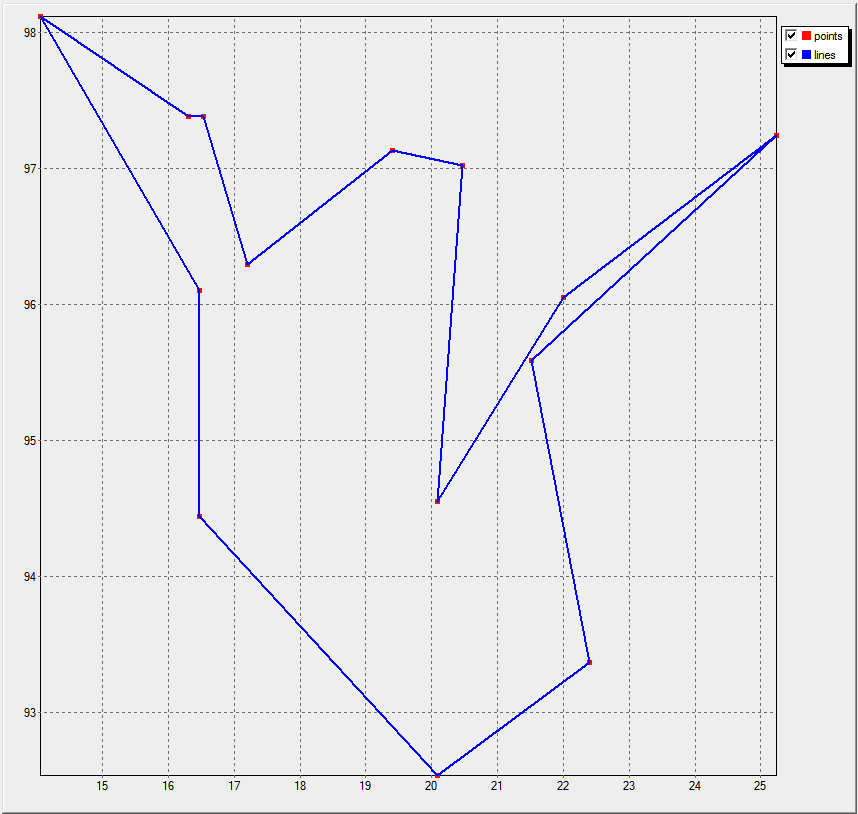
\includegraphics[width=\linewidth]{results-burma14-tm}
					\caption{Solución \emph{Exacta (TM)}}
				\end{subfigure} \
				\begin{subfigure}{.4\textwidth}
					\centering
					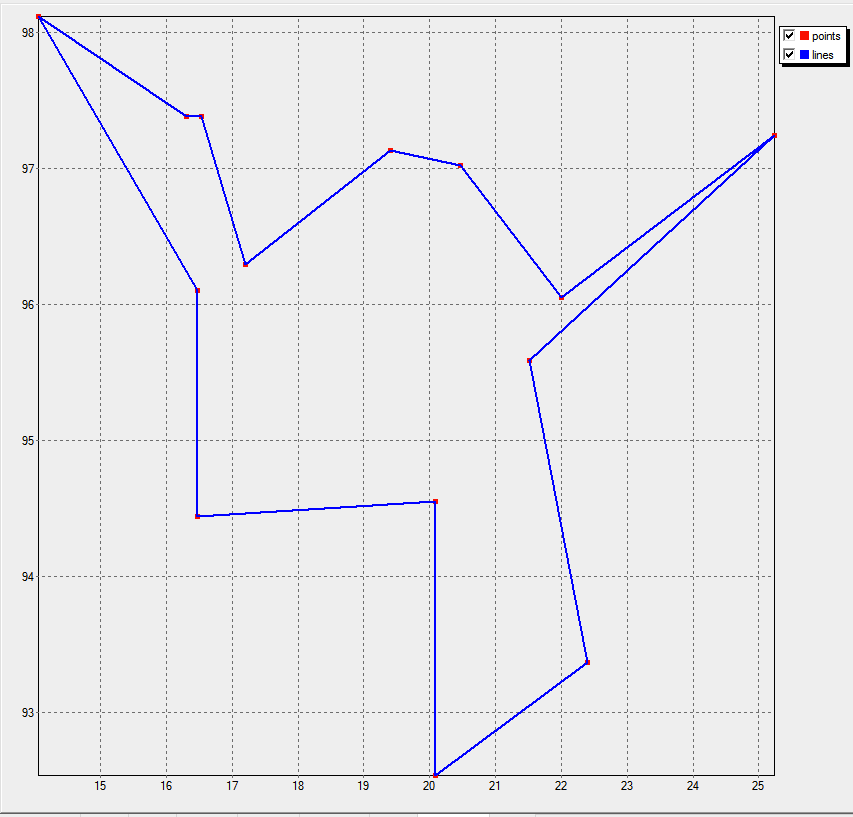
\includegraphics[width=\linewidth]{results-burma14-redes}
					\caption{Solución \emph{Entorno más Cercano (Redes)}}
				\end{subfigure}
				\caption{Representación gráfica de las distintas soluciones para el conjunto de datos \emph{burma14}}
				\label{fig:sol-burma14}
			\end{figure}


		\subsection{br17}

			\paragraph{}
			El conjunto de datos está formado por la matriz de distancias de $17$ nodos. En este caso se resuelve de manera exacta mediante la formulación de \emph{Tucker-Miller} y la de \emph{Redes}. Al igual que en el caso anterior, ambas soluciones son óptimas, sin embargo proporcionan caminos distintos. Los resultados se muestran en la tabla \ref{table:sol-br17}.

			\begin{table}[H]
				\centering
				\begin{tabu}{ | c | c | p{.65\linewidth} |}
					\hline
					\bfseries Método & \bfseries Distancia & \bfseries Camino
					\csvreader[head to column names]{../results/csv/results-br17.csv}{}
					{\\\hline\method&\distance&\path}
					\\\hline
				\end{tabu}
				\caption{Soluciones para el conjunto de datos \emph{br17}}
				\label{table:sol-br17}
			\end{table}

		\subsection{n21\_1}

			\paragraph{}
			El conjunto de datos está formado por la matriz de distancias de $21$ nodos. En este caso se ha resulto de manera exacta mediante la formulación de \emph{Tucker-Miller} y de manera aproximada mediante heurísticas \emph{Entorno más Cercano}, \emph{2-opt}, \emph{GRASP} y \emph{Simulated Anneling}. Los resultados se muestran en la tabla \ref{table:sol-n21_1}.

			\begin{table}[H]
				\centering
				\begin{tabu}{ | c | c | p{.65\linewidth} |}
					\hline
			   	\bfseries Método & \bfseries Distancia & \bfseries Camino
			    \csvreader[head to column names]{../results/csv/results-n21_1.csv}{}
			    {\\\hline\method&\distance&\path}
					\\\hline
		    \end{tabu}
				\caption{Soluciones para el conjunto de datos \emph{n21\_1}}
				\label{table:sol-n21_1}
			\end{table}

		\subsection{n21\_2}

			\paragraph{}
			El conjunto de datos está formado por la matriz de distancias de $21$ nodos. En este caso se ha resulto de manera exacta mediante la formulación de \emph{Tucker-Miller} y de manera aproximada mediante heurísticas \emph{Entorno más Cercano}, \emph{2-opt}, \emph{GRASP} y \emph{Simulated Anneling}. Los resultados se muestran en la tabla \ref{table:sol-n21_2}.

			\begin{table}[H]
				\centering
				\begin{tabu}{ | c | c | p{.65\linewidth} |}
					\hline
			   	\bfseries Método & \bfseries Distancia & \bfseries Camino
			    \csvreader[head to column names]{../results/csv/results-n21_2.csv}{}
			    {\\\hline\method&\distance&\path}
					\\\hline
		    \end{tabu}
				\caption{Soluciones para el conjunto de datos \emph{n21\_2}}
				\label{table:sol-n21_2}
			\end{table}

		\subsection{n21\_3}

			\paragraph{}
			El conjunto de datos está formado por la matriz de distancias de $21$ nodos. En este caso se ha resulto de manera exacta mediante la formulación de \emph{Tucker-Miller} y de manera aproximada mediante heurísticas \emph{Entorno más Cercano}, \emph{2-opt}, \emph{GRASP} y \emph{Simulated Anneling}. Los resultados se muestran en la tabla \ref{table:sol-n21_3}.

			\begin{table}[H]
				\centering
				\begin{tabu}{ | c | c | p{.65\linewidth} |}
					\hline
			   	\bfseries Método & \bfseries Distancia & \bfseries Camino
			    \csvreader[head to column names]{../results/csv/results-n21_3.csv}{}
			    {\\\hline\method&\distance&\path}
					\\\hline
		    \end{tabu}
				\caption{Soluciones para el conjunto de datos \emph{n21\_3}}
				\label{table:sol-n21_3}
			\end{table}

		\subsection{n21\_4}

			\paragraph{}
			El conjunto de datos está formado por la matriz de distancias de $21$ nodos. En este caso se ha resulto de manera exacta mediante la formulación de \emph{Tucker-Miller} y de manera aproximada mediante heurísticas \emph{Entorno más Cercano}, \emph{2-opt}, \emph{GRASP} y \emph{Simulated Anneling}. Los resultados se muestran en la tabla \ref{table:sol-n21_4}.

			\begin{table}[H]
				\centering
				\begin{tabu}{ | c | c | p{.65\linewidth} |}
					\hline
			   	\bfseries Método & \bfseries Distancia & \bfseries Camino
			    \csvreader[head to column names]{../results/csv/results-n21_4.csv}{}
			    {\\\hline\method&\distance&\path}
					\\\hline
		    \end{tabu}
				\caption{Soluciones para el conjunto de datos \emph{n21\_4}}
				\label{table:sol-n21_4}
			\end{table}

		\subsection{n21\_5}

			\paragraph{}
			El conjunto de datos está formado por la matriz de distancias de $21$ nodos. En este caso se ha resulto de manera exacta mediante la formulación de \emph{Tucker-Miller} y de manera aproximada mediante heurísticas \emph{Entorno más Cercano}, \emph{2-opt}, \emph{GRASP} y \emph{Simulated Anneling}. Los resultados se muestran en la tabla \ref{table:sol-n21_5}.

			\begin{table}[H]
				\centering
				\begin{tabu}{ | c | c | p{.65\linewidth} |}
					\hline
			   	\bfseries Método & \bfseries Distancia & \bfseries Camino
			    \csvreader[head to column names]{../results/csv/results-n21_5.csv}{}
			    {\\\hline\method&\distance&\path}
					\\\hline
		    \end{tabu}
				\caption{Soluciones para el conjunto de datos \emph{n21\_5}}
				\label{table:sol-n21_5}
			\end{table}

		\subsection{tsp\_60\_1}

			\paragraph{}
			El conjunto de datos está formado por las coordenadas de $60$ nodos (por lo que es necesario calcular las distancias previamente). En este caso se ha resulto de manera exacta mediante la formulación de \emph{Tucker-Miller} y de manera aproximada mediante heurísticas \emph{Entorno más Cercano}, \emph{2-opt}, \emph{GRASP} y \emph{Simulated Anneling}. En la tabla \ref{table:sol-tsp_60_1} se muestran los resultados de forma numérica mientras que en la figura \ref{fig:sol-tsp_60_1} se muestra la representación gráfica.

			\begin{table}[H]
				\centering
				\begin{tabu}{ | c | c | p{.65\linewidth} |}
					\hline
			   	\bfseries Método & \bfseries Distancia & \bfseries Camino
			    \csvreader[head to column names]{../results/csv/results-tsp_60_1.csv}{}
			    {\\\hline\method&\distance&\path}
					\\\hline
		    \end{tabu}
				\caption{Soluciones para el conjunto de datos \emph{tsp\_60\_1}}
				\label{table:sol-tsp_60_1}
			\end{table}


			\begin{figure}[h]
				\centering
				\begin{subfigure}{.4\textwidth}
					\centering
					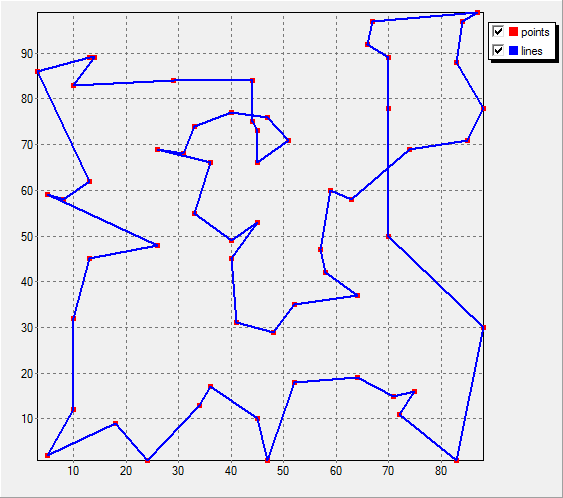
\includegraphics[width=\linewidth]{results-tsp_60_1-exact}
					\caption{Solución \emph{Exacta}}
				\end{subfigure} \
				\begin{subfigure}{.4\textwidth}
					\centering
					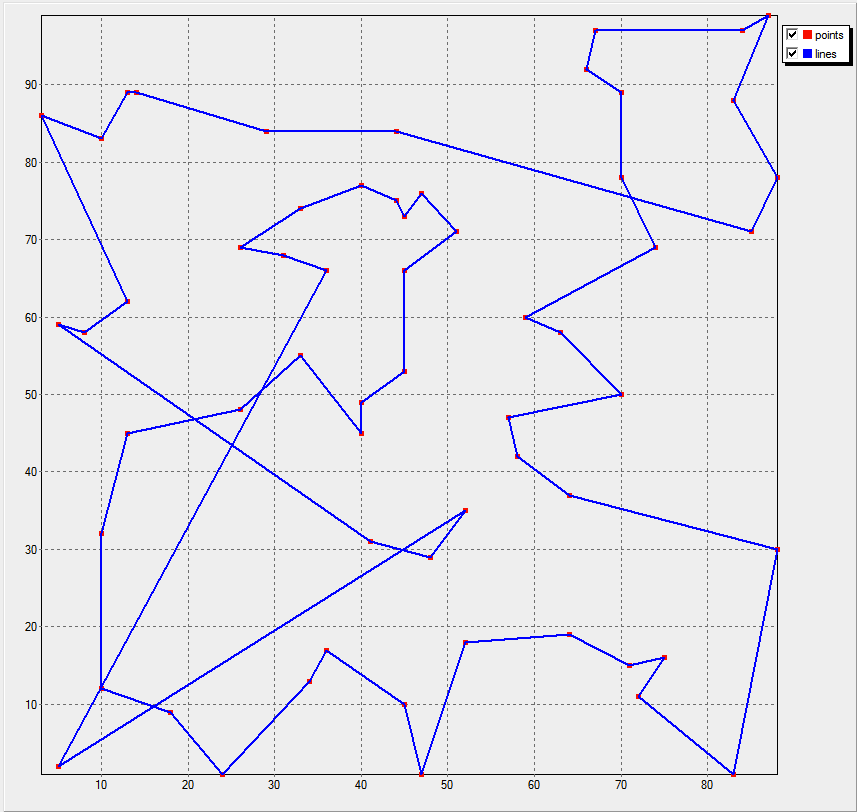
\includegraphics[width=\linewidth]{results-tsp_60_1-greedy}
					\caption{Solución \emph{Entorno más Cercano}}
				\end{subfigure} \\
				\begin{subfigure}{.4\textwidth}
					\centering
					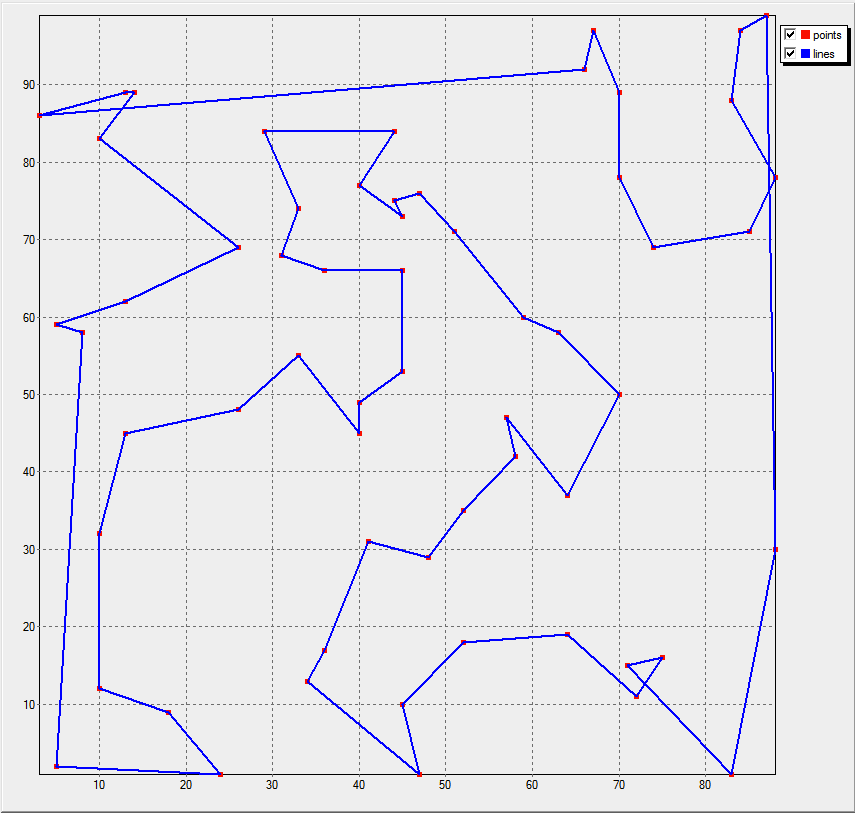
\includegraphics[width=\linewidth]{results-tsp_60_1-opt}
					\caption{Solución \emph{2-opt}}
				\end{subfigure} \
				\begin{subfigure}{.4\textwidth}
					\centering
					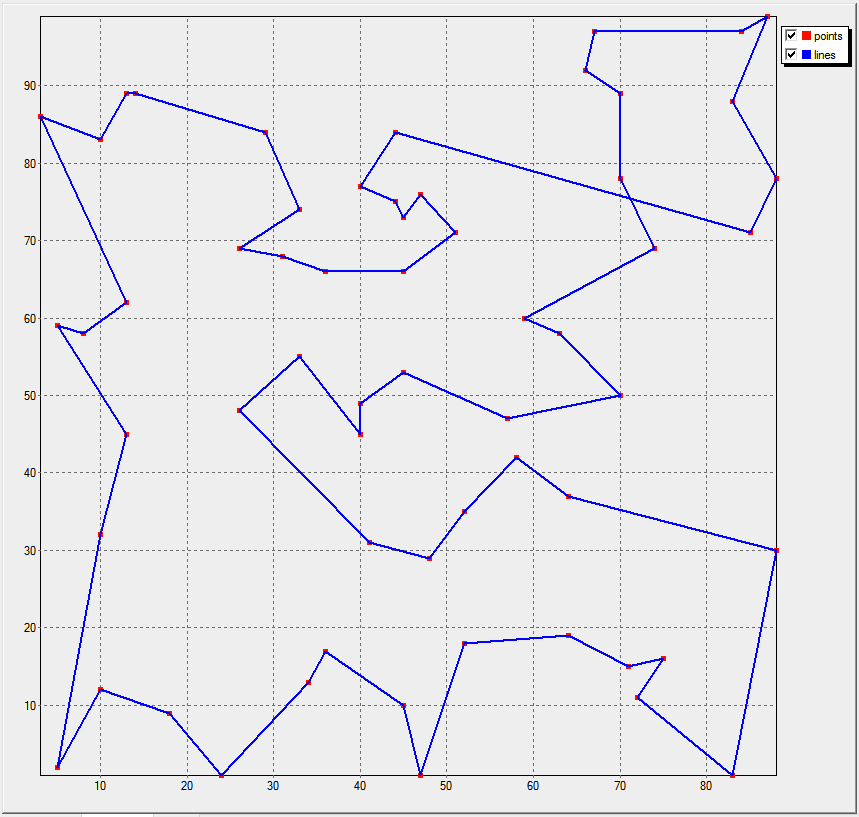
\includegraphics[width=\linewidth]{results-tsp_60_1-grasp}
					\caption{Solución \emph{GRASP}}
				\end{subfigure} \\
				\begin{subfigure}{.4\textwidth}
					\centering
					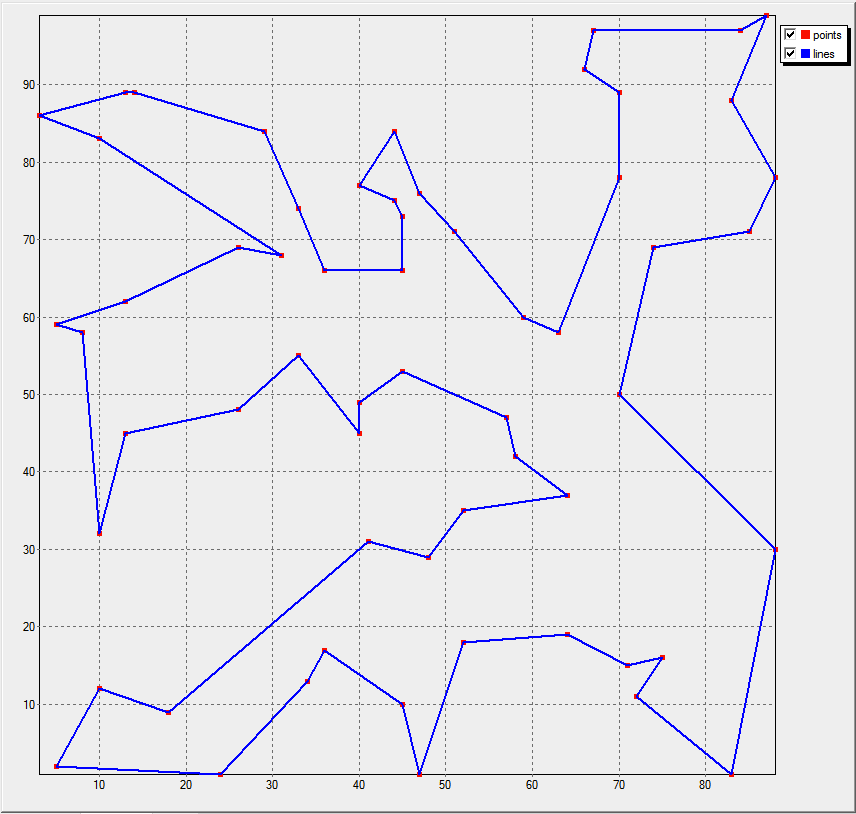
\includegraphics[width=\linewidth]{results-tsp_60_1-sa}
					\caption{Solución \emph{Simulated Anneling}}
				\end{subfigure}
				\caption{Representación gráfica de las distintas soluciones para el conjunto de datos \emph{tsp\_60\_1}}
				\label{fig:sol-tsp_60_1}
			\end{figure}


		\subsection{tsp\_60\_2}

			\paragraph{}
			El conjunto de datos está formado por las coordenadas de $60$ nodos (por lo que es necesario calcular las distancias previamente). En este caso se ha resulto de manera exacta mediante la formulación de \emph{Tucker-Miller} y de manera aproximada mediante heurísticas \emph{Entorno más Cercano}, \emph{2-opt}, \emph{GRASP} y \emph{Simulated Anneling}. En la tabla \ref{table:sol-tsp_60_2} se muestran los resultados de forma numérica mientras que en la figura \ref{fig:sol-tsp_60_2} se muestra la representación gráfica.

			\begin{table}[H]
				\centering
				\begin{tabu}{ | c | c | p{.65\linewidth} |}
					\hline
			   	\bfseries Método & \bfseries Distancia & \bfseries Camino
			    \csvreader[head to column names]{../results/csv/results-tsp_60_2.csv}{}
			    {\\\hline\method&\distance&\path}
					\\\hline
		    \end{tabu}
				\caption{Soluciones para el conjunto de datos \emph{tsp\_60\_2}}
				\label{table:sol-tsp_60_2}
			\end{table}

			\begin{figure}[h]
				\centering
				\begin{subfigure}{.4\textwidth}
					\centering
					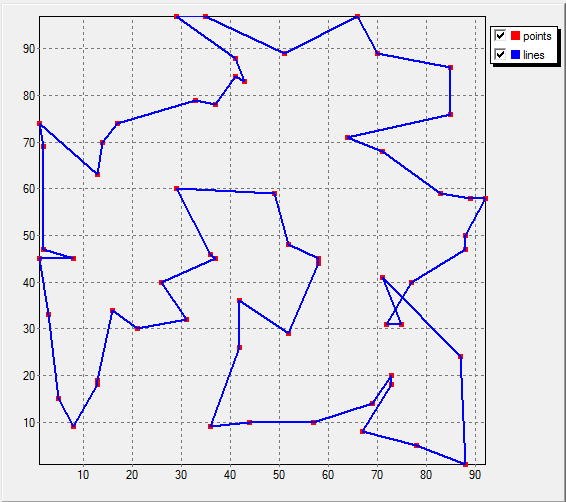
\includegraphics[width=\linewidth]{results-tsp_60_2-exact}
					\caption{Solución \emph{Exacta}}
				\end{subfigure} \
				\begin{subfigure}{.4\textwidth}
					\centering
					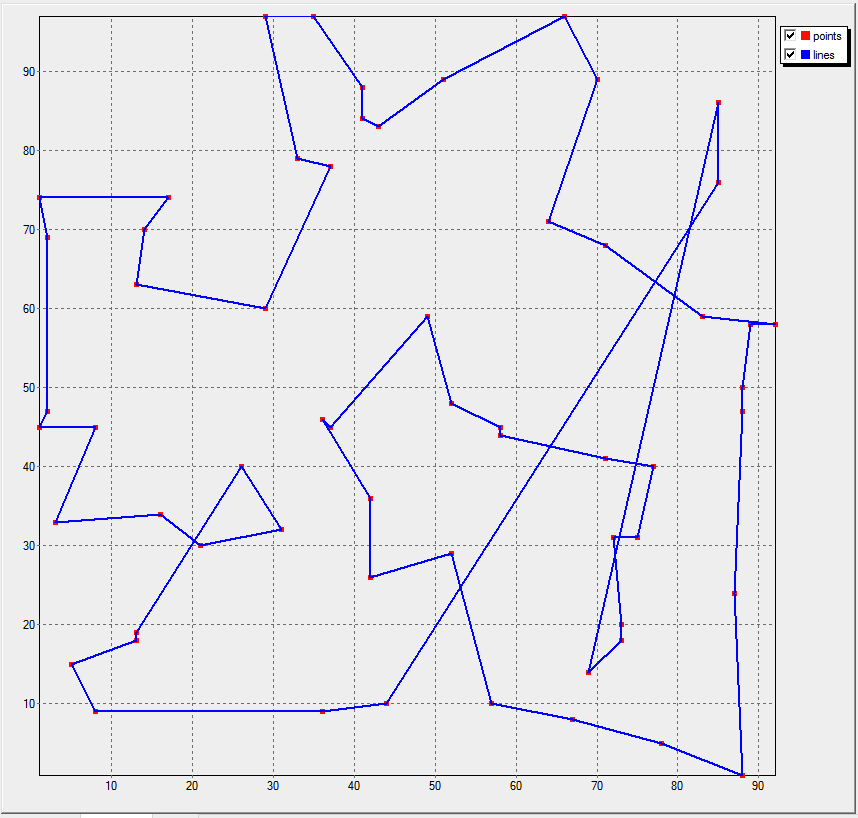
\includegraphics[width=\linewidth]{results-tsp_60_2-greedy}
					\caption{Solución \emph{Entorno más Cercano}}
				\end{subfigure} \\
				\begin{subfigure}{.4\textwidth}
					\centering
					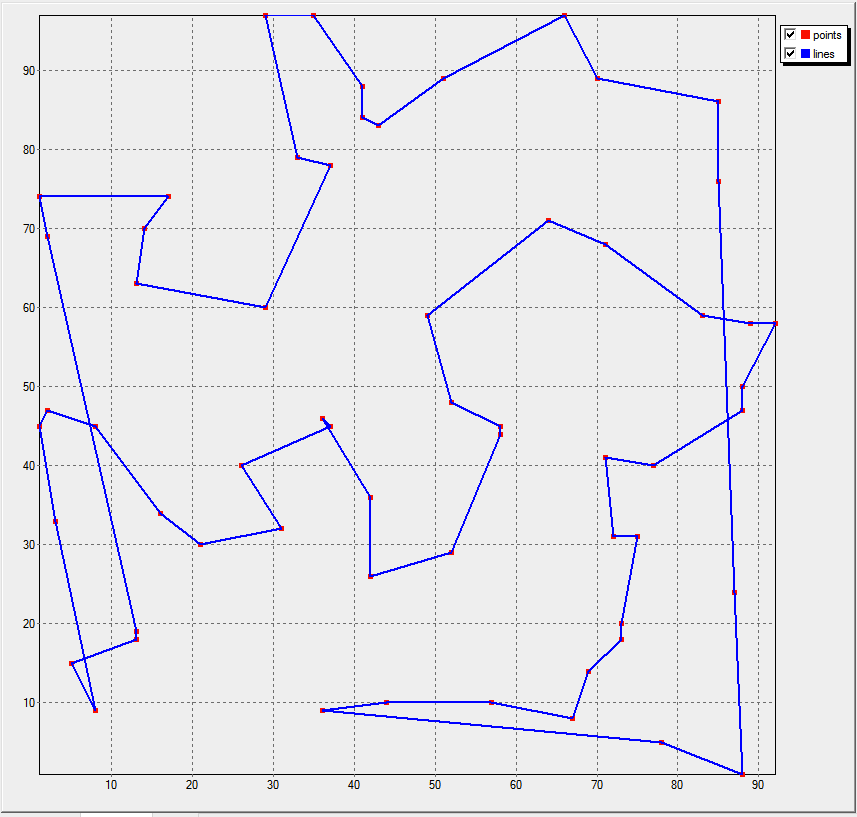
\includegraphics[width=\linewidth]{results-tsp_60_2-opt}
					\caption{Solución \emph{2-opt}}
				\end{subfigure} \
				\begin{subfigure}{.4\textwidth}
					\centering
					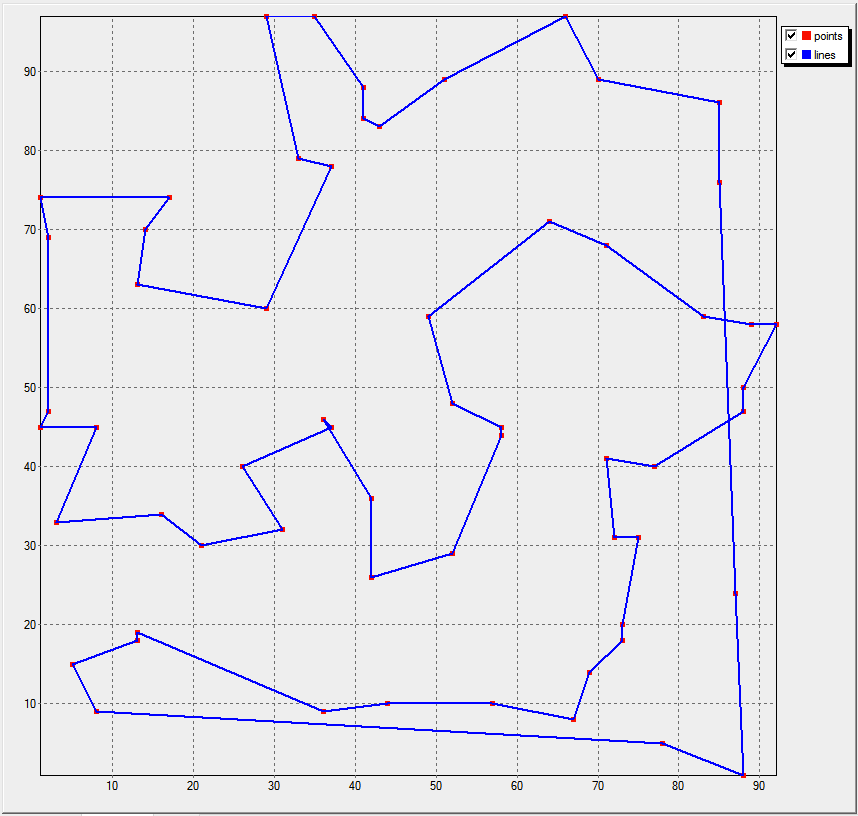
\includegraphics[width=\linewidth]{results-tsp_60_2-grasp}
					\caption{Solución \emph{GRASP}}
				\end{subfigure} \\
				\begin{subfigure}{.4\textwidth}
					\centering
					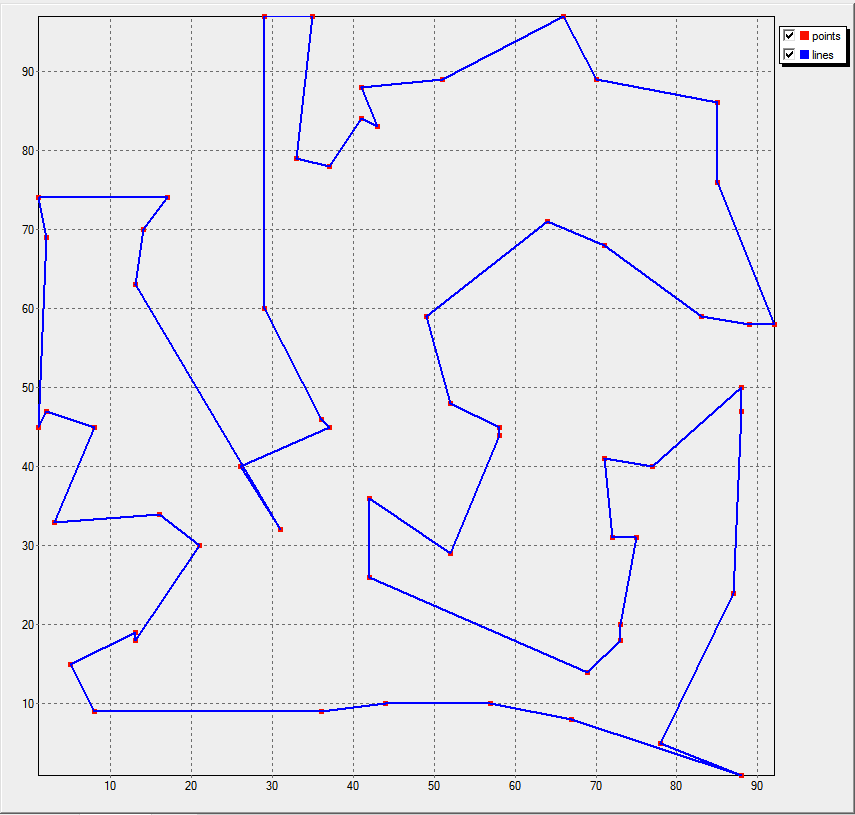
\includegraphics[width=\linewidth]{results-tsp_60_2-sa}
					\caption{Solución \emph{Simulated Anneling}}
				\end{subfigure}
				\caption{Representación gráfica de las distintas soluciones para el conjunto de datos \emph{tsp\_60\_2}}
				\label{fig:sol-tsp_60_2}
			\end{figure}

		\subsection{tsp\_60\_3}

			\paragraph{}
			El conjunto de datos está formado por las coordenadas de $60$ nodos (por lo que es necesario calcular las distancias previamente). En este caso se ha resulto de manera exacta mediante la formulación de \emph{Tucker-Miller} y de manera aproximada mediante heurísticas \emph{Entorno más Cercano}, \emph{2-opt}, \emph{GRASP} y \emph{Simulated Anneling}. En la tabla \ref{table:sol-tsp_60_3} se muestran los resultados de forma numérica mientras que en la figura \ref{fig:sol-tsp_60_3} se muestra la representación gráfica.

			\begin{table}[H]
				\centering
				\begin{tabu}{ | c | c | p{.65\linewidth} |}
					\hline
			   	\bfseries Método & \bfseries Distancia & \bfseries Camino
			    \csvreader[head to column names]{../results/csv/results-tsp_60_3.csv}{}
			    {\\\hline\method&\distance&\path}
					\\\hline
		    \end{tabu}
				\caption{Soluciones para el conjunto de datos \emph{tsp\_60\_3}}
				\label{table:sol-tsp_60_3}
			\end{table}

			\begin{figure}[h]
				\centering
				\begin{subfigure}{.4\textwidth}
					\centering
					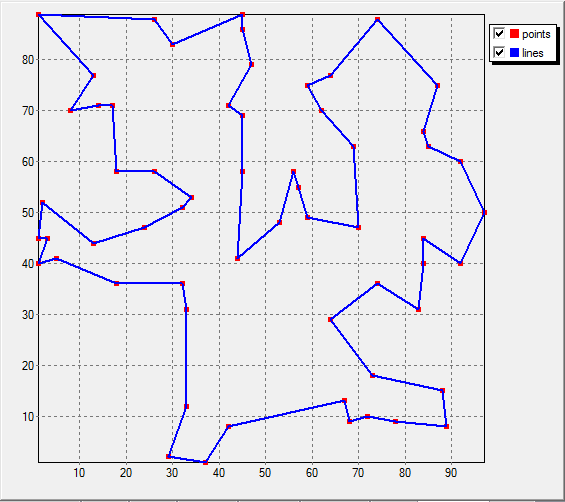
\includegraphics[width=\linewidth]{results-tsp_60_3-exact}
					\caption{Solución \emph{Exacta}}
				\end{subfigure} \
				\begin{subfigure}{.4\textwidth}
					\centering
					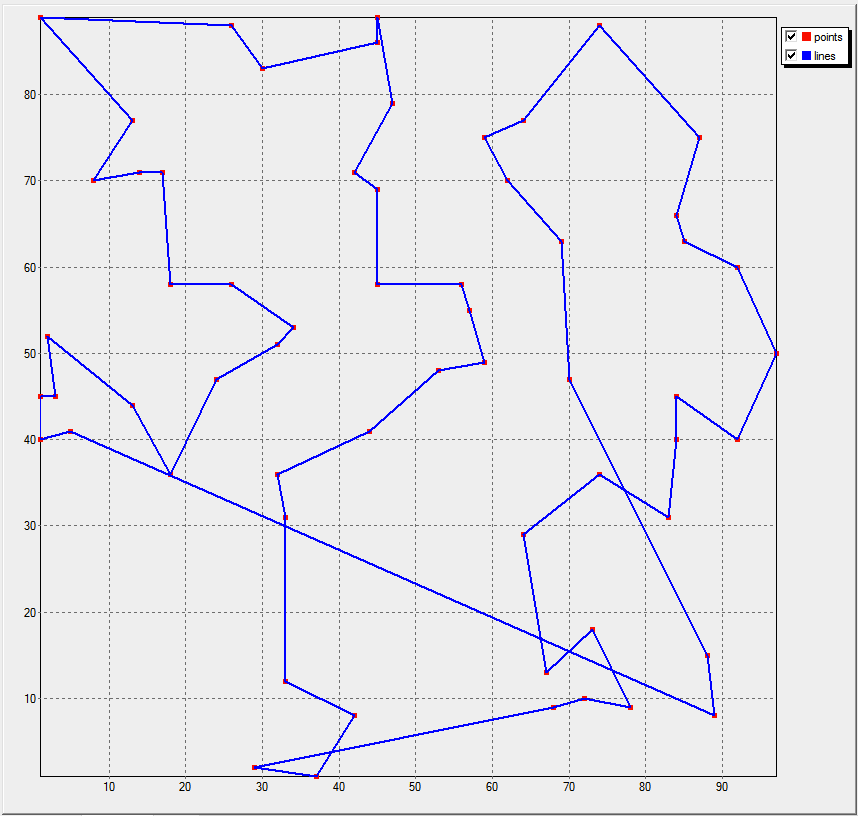
\includegraphics[width=\linewidth]{results-tsp_60_3-greedy}
					\caption{Solución \emph{Entorno más Cercano}}
				\end{subfigure} \\
				\begin{subfigure}{.4\textwidth}
					\centering
					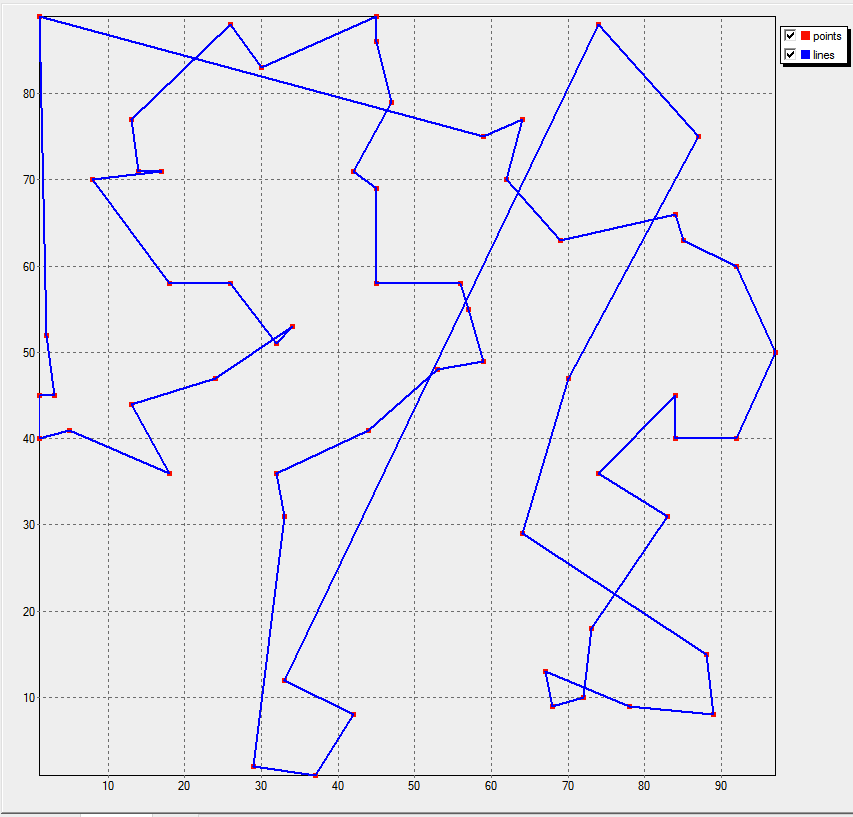
\includegraphics[width=\linewidth]{results-tsp_60_3-opt}
					\caption{Solución \emph{2-opt}}
				\end{subfigure} \
				\begin{subfigure}{.4\textwidth}
					\centering
					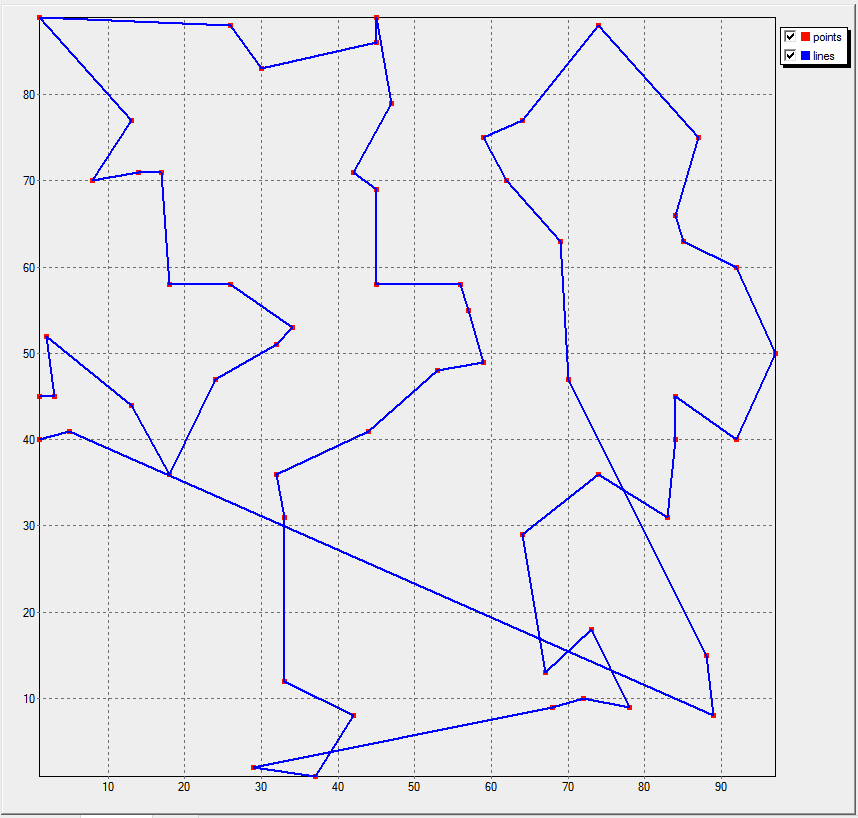
\includegraphics[width=\linewidth]{results-tsp_60_3-grasp}
					\caption{Solución \emph{GRASP}}
				\end{subfigure} \\
				\begin{subfigure}{.4\textwidth}
					\centering
					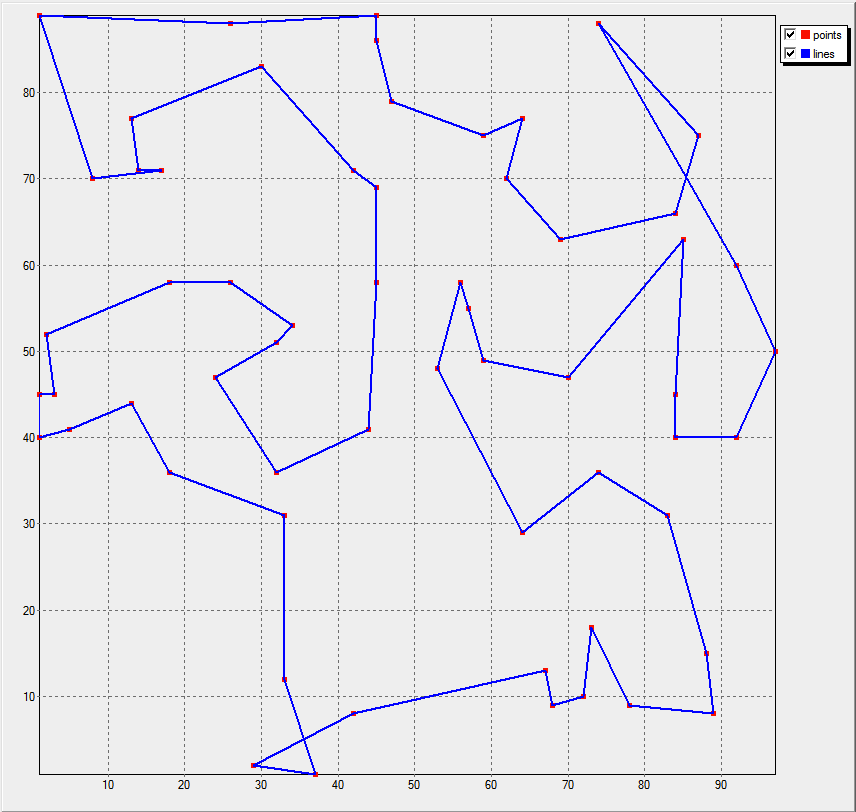
\includegraphics[width=\linewidth]{results-tsp_60_3-sa}
					\caption{Solución \emph{Simulated Anneling}}
				\end{subfigure}
				\caption{Representación gráfica de las distintas soluciones para el conjunto de datos \emph{tsp\_60\_3}}
				\label{fig:sol-tsp_60_3}
			\end{figure}

		\subsection{tsp\_100\_1}

			\paragraph{}
			El conjunto de datos está formado por las coordenadas de $100$ nodos (por lo que es necesario calcular las distancias previamente). En este caso se ha resulto de manera exacta mediante la formulación de \emph{Tucker-Miller} y de manera aproximada mediante heurísticas \emph{Entorno más Cercano}, \emph{2-opt}, \emph{GRASP} y \emph{Simulated Anneling}. En la tabla \ref{table:sol-tsp_100_1} se muestran los resultados de forma numérica mientras que en la figura \ref{fig:sol-tsp_100_1} se muestra la representación gráfica.

			\begin{table}[H]
				\centering
				\begin{tabu}{ | c | c | p{.65\linewidth} |}
					\hline
			   	\bfseries Método & \bfseries Distancia & \bfseries Camino
			    \csvreader[head to column names]{../results/csv/results-tsp_100_1.csv}{}
			    {\\\hline\method&\distance&\path}
					\\\hline
		    \end{tabu}
				\caption{Soluciones para el conjunto de datos \emph{tsp\_100\_1}}
				\label{table:sol-tsp_100_1}
			\end{table}

			\begin{figure}[h]
				\centering
				\begin{subfigure}{.4\textwidth}
					\centering
					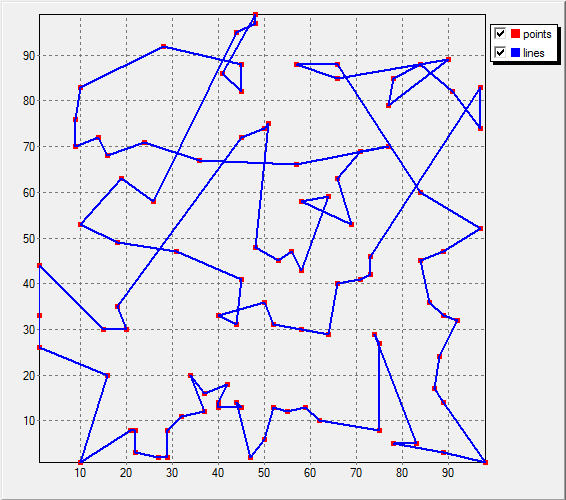
\includegraphics[width=\linewidth]{results-tsp_100_1-exact}
					\caption{Solución \emph{Exacta}}
				\end{subfigure} \
				\begin{subfigure}{.4\textwidth}
					\centering
					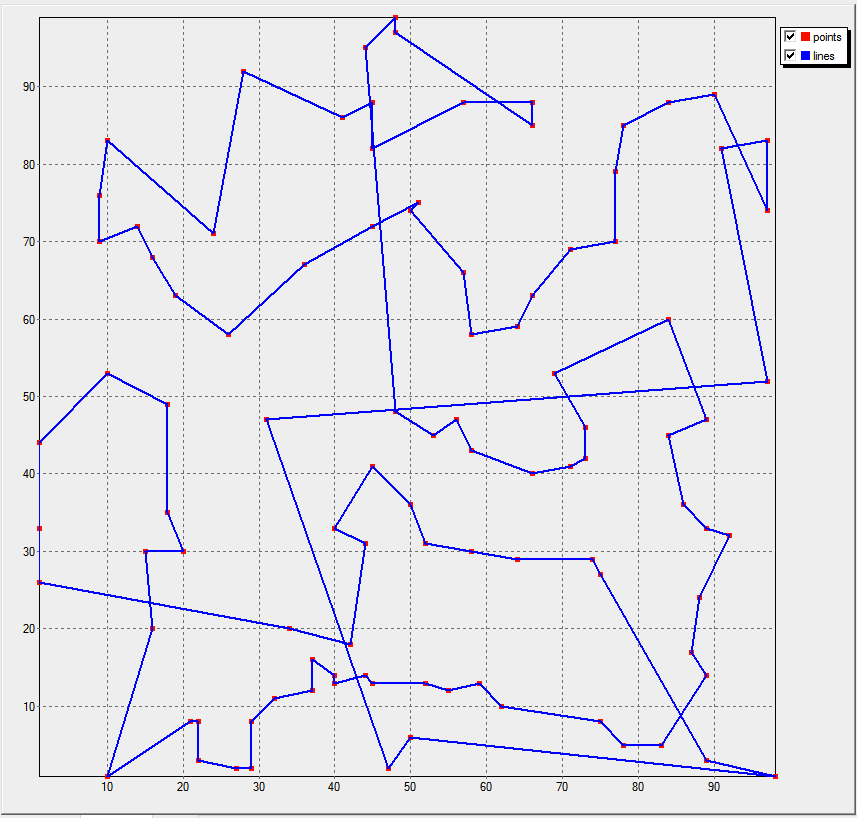
\includegraphics[width=\linewidth]{results-tsp_100_1-greedy}
					\caption{Solución \emph{Entorno más Cercano}}
				\end{subfigure} \\
				\begin{subfigure}{.4\textwidth}
					\centering
					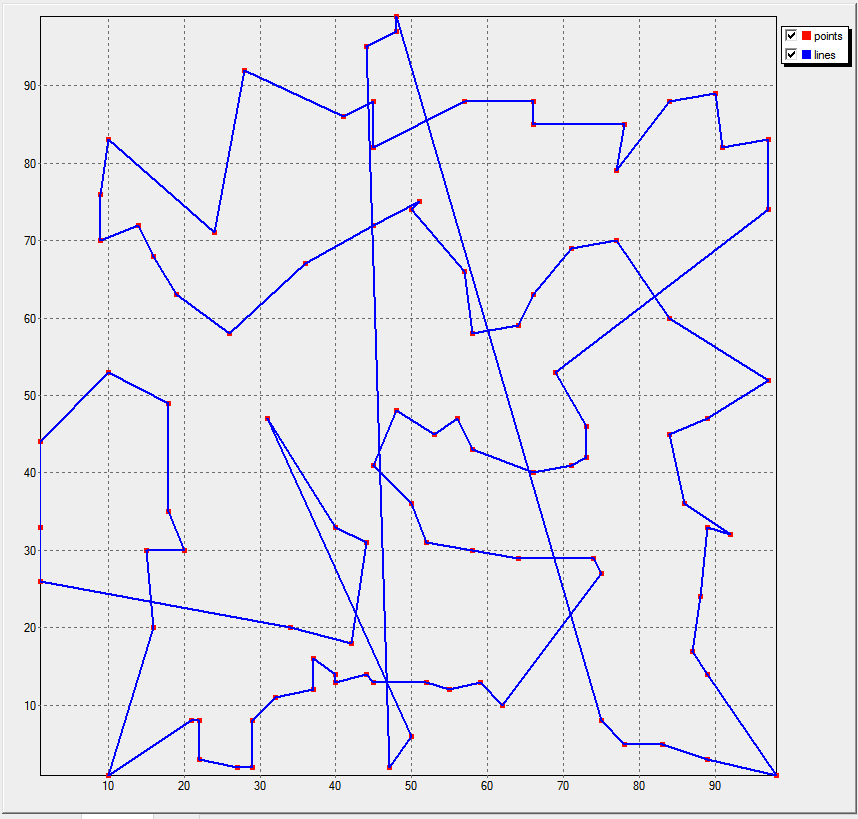
\includegraphics[width=\linewidth]{results-tsp_100_1-opt}
					\caption{Solución \emph{2-opt}}
				\end{subfigure} \
				\begin{subfigure}{.4\textwidth}
					\centering
					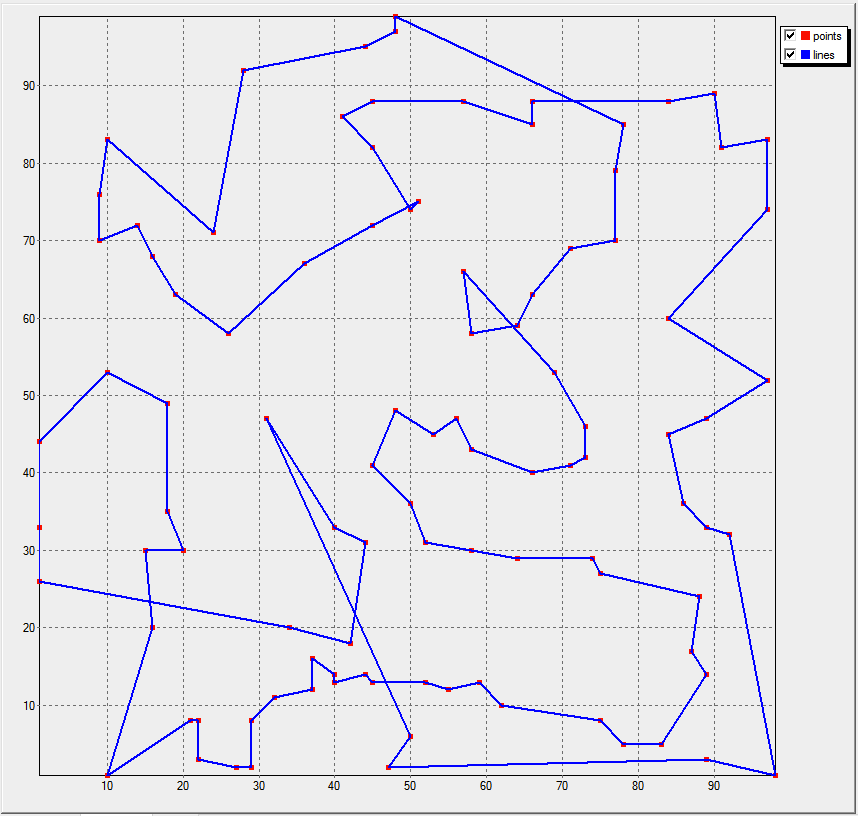
\includegraphics[width=\linewidth]{results-tsp_100_1-grasp}
					\caption{Solución \emph{GRASP}}
				\end{subfigure} \\
				\begin{subfigure}{.4\textwidth}
					\centering
					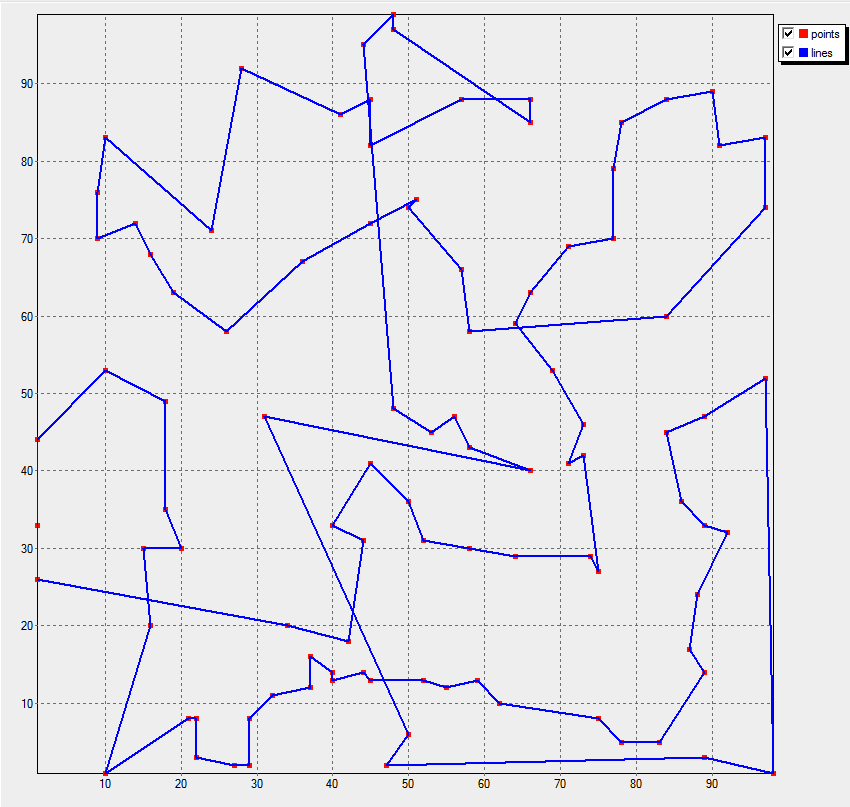
\includegraphics[width=\linewidth]{results-tsp_100_1-sa}
					\caption{Solución \emph{Simulated Anneling}}
				\end{subfigure}
				\caption{Representación gráfica de las distintas soluciones para el conjunto de datos \emph{tsp\_100\_1}}
				\label{fig:sol-tsp_100_1}
			\end{figure}

		\subsection{tsp\_100\_2}

			\paragraph{}
			El conjunto de datos está formado por las coordenadas de $100$ nodos (por lo que es necesario calcular las distancias previamente). En este caso se ha resulto de manera exacta mediante la formulación de \emph{Tucker-Miller} y de manera aproximada mediante heurísticas \emph{Entorno más Cercano}, \emph{2-opt}, \emph{GRASP} y \emph{Simulated Anneling}. En la tabla \ref{table:sol-tsp_100_2} se muestran los resultados de forma numérica mientras que en la figura \ref{fig:sol-tsp_100_2} se muestra la representación gráfica.

			\begin{table}[H]
				\centering
				\begin{tabu}{ | c | c | p{.65\linewidth} |}
					\hline
					\bfseries Método & \bfseries Distancia & \bfseries Camino
					\csvreader[head to column names]{../results/csv/results-tsp_100_2.csv}{}
					{\\\hline\method&\distance&\path}
					\\\hline
				\end{tabu}
				\caption{Soluciones para el conjunto de datos \emph{tsp\_100\_2}}
				\label{table:sol-tsp_100_2}
			\end{table}

			\begin{figure}[h]
				\centering
				\begin{subfigure}{.4\textwidth}
					\centering
					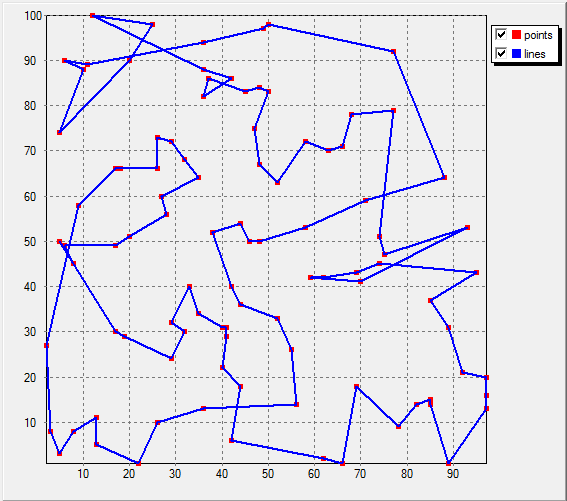
\includegraphics[width=\linewidth]{results-tsp_100_2-exact}
					\caption{Solución \emph{Exacta}}
				\end{subfigure} \
				\begin{subfigure}{.4\textwidth}
					\centering
					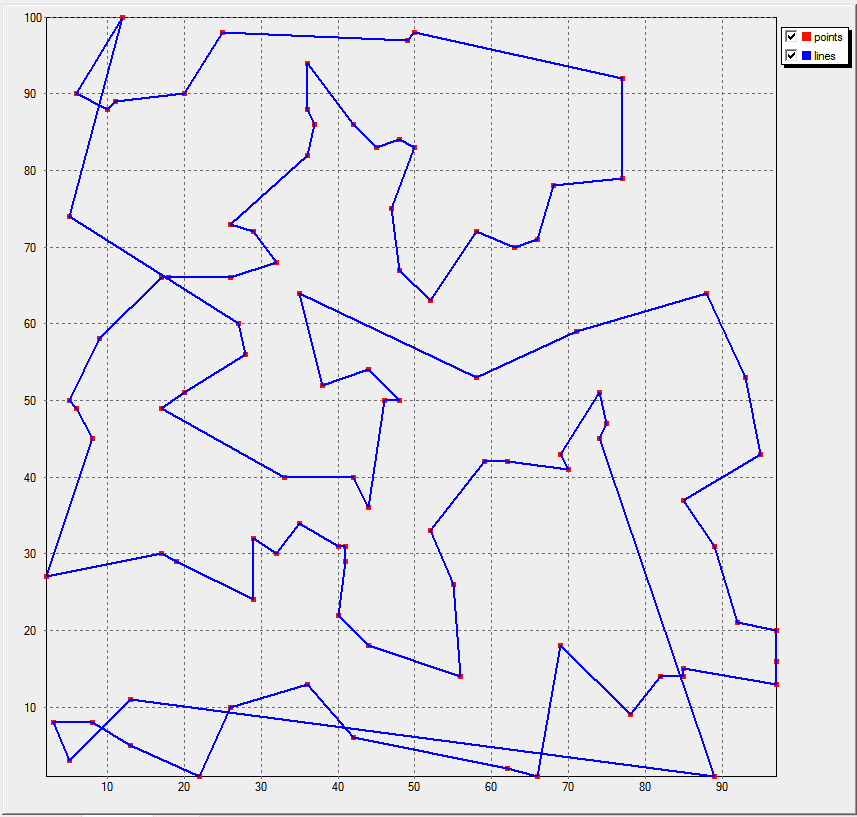
\includegraphics[width=\linewidth]{results-tsp_100_2-greedy}
					\caption{Solución \emph{Entorno más Cercano}}
				\end{subfigure} \\
				\begin{subfigure}{.4\textwidth}
					\centering
					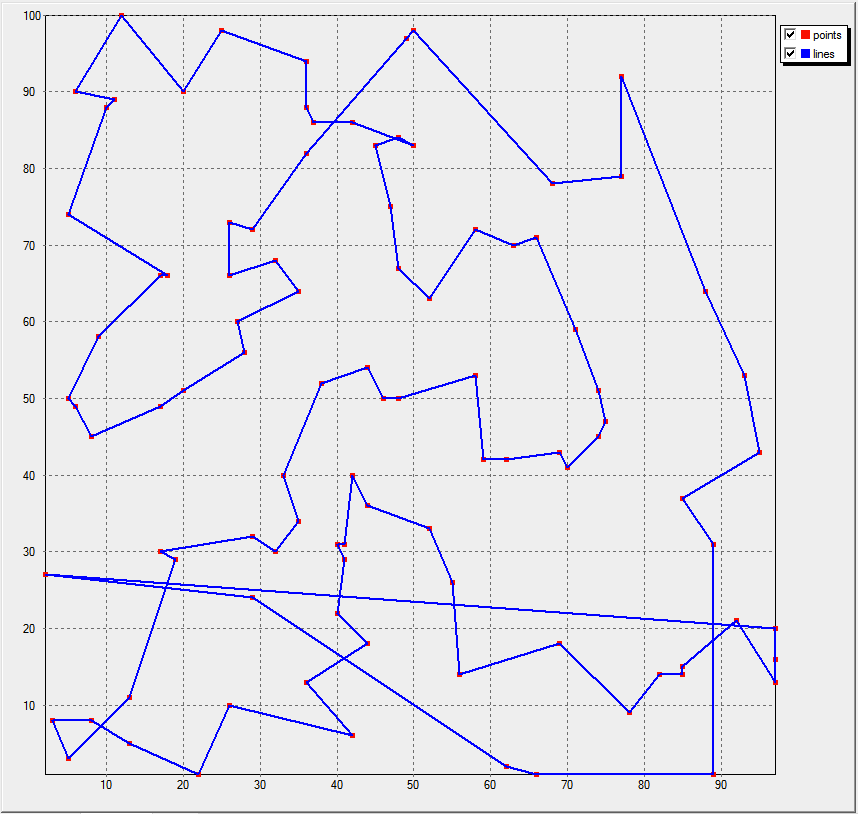
\includegraphics[width=\linewidth]{results-tsp_100_2-opt}
					\caption{Solución \emph{2-opt}}
				\end{subfigure} \
				\begin{subfigure}{.4\textwidth}
					\centering
					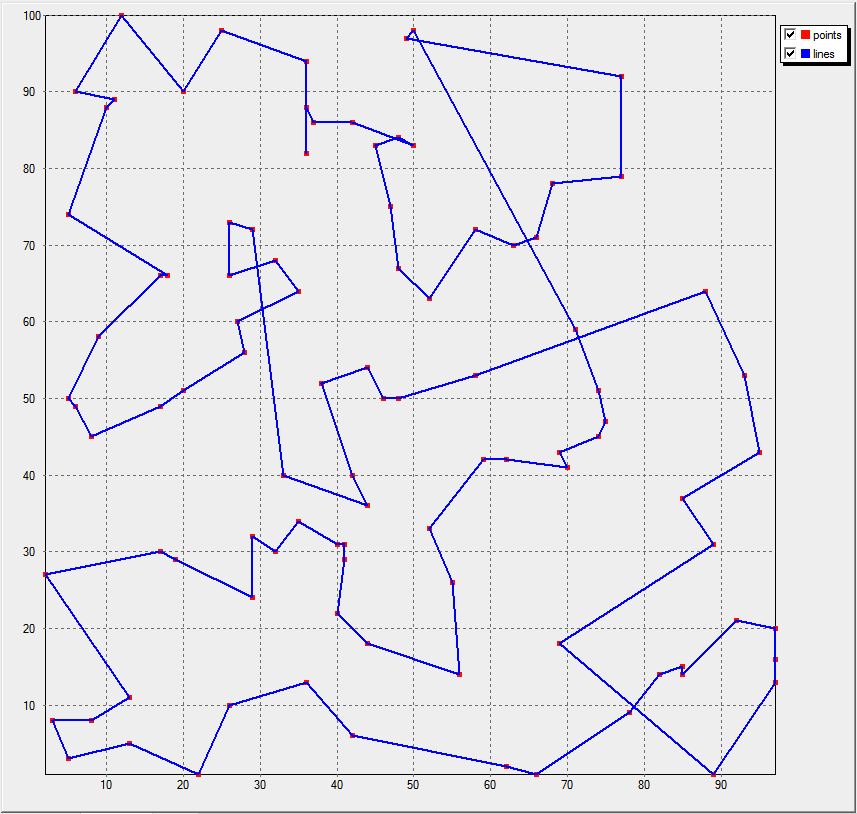
\includegraphics[width=\linewidth]{results-tsp_100_2-grasp}
					\caption{Solución \emph{GRASP}}
				\end{subfigure} \\
				\begin{subfigure}{.4\textwidth}
					\centering
					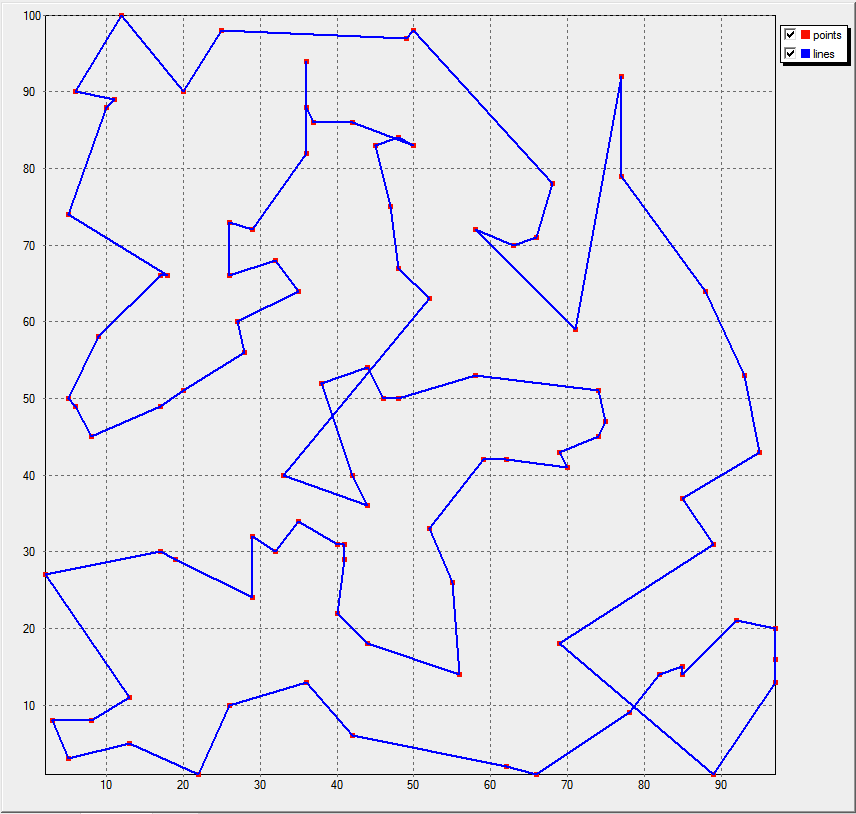
\includegraphics[width=\linewidth]{results-tsp_100_2-sa}
					\caption{Solución \emph{Simulated Anneling}}
				\end{subfigure}
				\caption{Representación gráfica de las distintas soluciones para el conjunto de datos \emph{tsp\_100\_2}}
				\label{fig:sol-tsp_100_2}
			\end{figure}

		\subsection{tsp\_100\_3}

			\paragraph{}
			El conjunto de datos está formado por las coordenadas de $100$ nodos (por lo que es necesario calcular las distancias previamente). En este caso se ha resulto de manera exacta mediante la formulación de \emph{Tucker-Miller} y de manera aproximada mediante heurísticas \emph{Entorno más Cercano}, \emph{2-opt}, \emph{GRASP} y \emph{Simulated Anneling}. En la tabla \ref{table:sol-tsp_100_3} se muestran los resultados de forma numérica mientras que en la figura \ref{fig:sol-tsp_100_3} se muestra la representación gráfica.

			\begin{table}[H]
				\centering
				\begin{tabu}{ | c | c | p{.65\linewidth} |}
					\hline
					\bfseries Método & \bfseries Distancia & \bfseries Camino
					\csvreader[head to column names]{../results/csv/results-tsp_100_3.csv}{}
					{\\\hline\method&\distance&\path}
					\\\hline
				\end{tabu}
				\caption{Soluciones para el conjunto de datos \emph{tsp\_100\_3}}
				\label{table:sol-tsp_100_3}
			\end{table}

			\begin{figure}[h]
				\centering
				\begin{subfigure}{.4\textwidth}
					\centering
					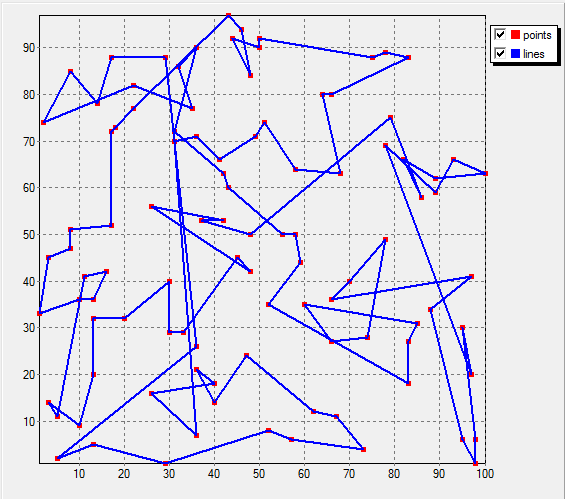
\includegraphics[width=\linewidth]{results-tsp_100_3-exact}
					\caption{Solución \emph{Exacta}}
				\end{subfigure} \
				\begin{subfigure}{.4\textwidth}
					\centering
					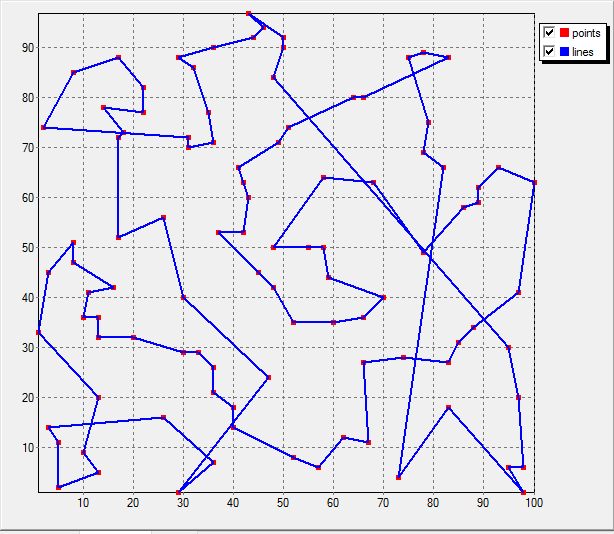
\includegraphics[width=\linewidth]{results-tsp_100_3-greedy}
					\caption{Solución \emph{Entorno más Cercano}}
				\end{subfigure} \\
				\begin{subfigure}{.4\textwidth}
					\centering
					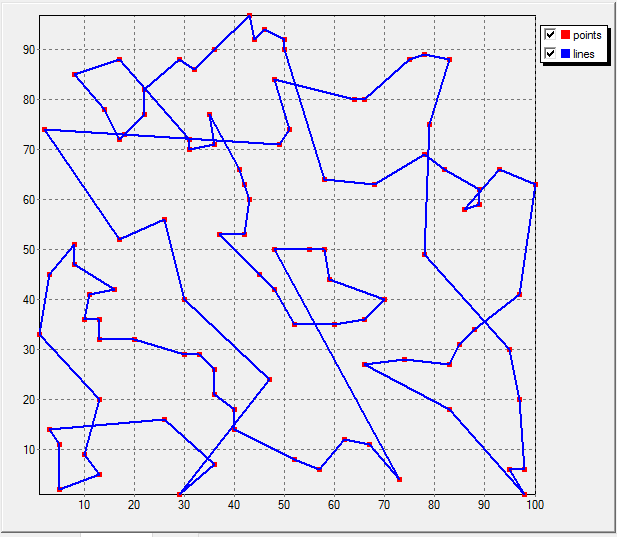
\includegraphics[width=\linewidth]{results-tsp_100_3-opt}
					\caption{Solución \emph{2-opt}}
				\end{subfigure} \
				\begin{subfigure}{.4\textwidth}
					\centering
					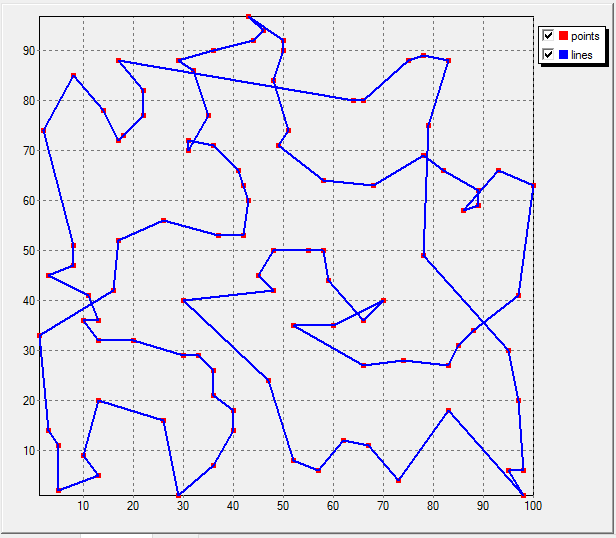
\includegraphics[width=\linewidth]{results-tsp_100_3-grasp}
					\caption{Solución \emph{GRASP}}
				\end{subfigure} \\
				\begin{subfigure}{.4\textwidth}
					\centering
					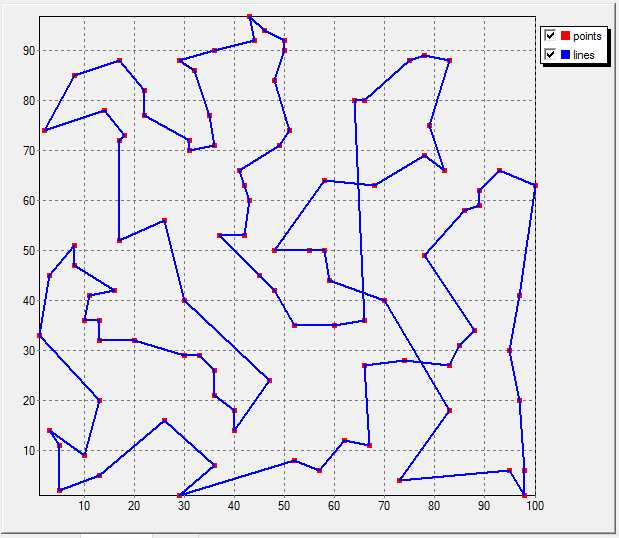
\includegraphics[width=\linewidth]{results-tsp_100_3-sa}
					\caption{Solución \emph{Simulated Anneling}}
				\end{subfigure}
				\caption{Representación gráfica de las distintas soluciones para el conjunto de datos \emph{tsp\_100\_3}}
				\label{fig:sol-tsp_100_3}
			\end{figure}

		\subsection{n40w20.001}

			\paragraph{}
			El conjunto de datos está formado por la matriz de distancias de $41$ nodos junto con sus correspondientes ventanas de tiempo. En este caso se ha resulto de manera exacta mediante la formulación de \emph{Tucker-Miller} añadiendo las correspondientes restricciones \emph{beta}($\beta$) referidas a las ventanas de tiempo. Los resultados se muestran en la tabla \ref{table:sol-n40w20.001}.

			\begin{table}[H]
				\centering
				\begin{tabu}{ | c | c | p{.65\linewidth} |}
					\hline
			   	\bfseries Método & \bfseries Distancia & \bfseries Camino
			    \csvreader[head to column names]{../results/csv/results-n40w20.001.csv}{}
			    {\\\hline\method&\distance&\path}
					\\\hline
		    \end{tabu}
				\caption{Soluciones para el conjunto de datos \emph{n40w20.001}}
				\label{table:sol-n40w20.001}
			\end{table}

		\subsection{n40w20.004}

			\paragraph{}
			El conjunto de datos está formado por la matriz de distancias de $41$ nodos junto con sus correspondientes ventanas de tiempo. En este caso se ha resulto de manera exacta mediante la formulación de \emph{Tucker-Miller} añadiendo las correspondientes restricciones \emph{beta}($\beta$) referidas a las ventanas de tiempo. Los resultados se muestran en la tabla \ref{table:sol-n40w20.004}.

			\begin{table}[H]
				\centering
				\begin{tabu}{ | c | c | p{.65\linewidth} |}
					\hline
			   	\bfseries Método & \bfseries Distancia & \bfseries Camino
			    \csvreader[head to column names]{../results/csv/results-n40w20.004.csv}{}
			    {\\\hline\method&\distance&\path}
					\\\hline
		    \end{tabu}
				\caption{Soluciones para el conjunto de datos \emph{n40w20.004}}
				\label{table:sol-n40w20.004}
			\end{table}

		\subsection{n60w20.005}

			\paragraph{}
			El conjunto de datos está formado por la matriz de distancias de $61$ nodos junto con sus correspondientes ventanas de tiempo. En este caso se ha resulto de manera exacta mediante la formulación de \emph{Tucker-Miller} añadiendo las correspondientes restricciones \emph{beta}($\beta$) referidas a las ventanas de tiempo. Los resultados se muestran en la tabla \ref{table:sol-n60w20.005}.

			\begin{table}[H]
				\centering
				\begin{tabu}{ | c | c | p{.65\linewidth} |}
					\hline
			   	\bfseries Método & \bfseries Distancia & \bfseries Camino
			    \csvreader[head to column names]{../results/csv/results-n60w20.005.csv}{}
			    {\\\hline\method&\distance&\path}
					\\\hline
		    \end{tabu}
				\caption{Soluciones para el conjunto de datos \emph{n60w20.005}}
				\label{table:sol-n60w20.005}
			\end{table}


%-----------------------------
%	BIBLIOGRAPHY
%-----------------------------
	\nocite{subject:mio}
	\nocite{garciparedes:mosel-examples}
	\bibliographystyle{acm}
  \bibliography{bib/misc}

\end{document}
